\chapter{搜索引擎优化}
\label{cha:filter}
\newcommand{\SmartDebug}{
	\textbf{\textit{SmartDebug}}
}

\section{引言}%2
在“生成-检验”系统中,搜索引擎负责生成程序变体,最终将其交由检验模块来验证该变体是否能够通过测试集。在搜索引擎模块的设计中,搜索空间的规划以及搜索算法直接影响系统整体的修复正确率和运行速度。采取一个广大的搜索空间可以提高系统的修复正确率,但是也意味着需要搜查的范围扩大,系统运行速度降低。因此,提高搜索算法的效率可以使得系统在可接受的时间范围内能够搜索到的空间更大,使得提高修复正确率成为可能。

现有系统的搜索算法可以分为两大类。第一类是基于构造或程序综合方法精准的生成程序变体。算法首先确定程序变体的基本结构,如需要替换表达式的具体位置和语法类型,接着利用静态分析、符号执行等技术,结合“程序变体需通过测试集中的所有测试”这一要求,生成逻辑公式描述替换表达式所应满足的语义要求,最后构造或利用程序综合技术直接生成满足要求的表达式。这一方法的优点在于“精确”,即理论上最终生成的表达式一定是满足逻辑公式要求的,因此将其替换进程序所生成的程序变体应直接通过测试集,几乎不需要再经过检验模块的验证。然而实际系统实现时我们会发现,生成逻辑公式这一过程非常耗时,因此将该算法应用于大规模程序有一定的难度。

另一类搜索算法基于预定义的修改模板生成程序变体。搜索算法首先在引擎内部预设了一组修改模板,用于描述在某些代码上下文中可能出现的错误情形以及相应的程序变体生成方法。例如,模板空指针检查器(Null-Checker)用以消除空指针错误,其内容是在某个指针的解引用前(上下文),插入一个判断指针是否为空的检查语句(变体生成方法)。依照这些模板,搜索算法能够针对不同的程序上下文生成合理的程序变体。因此,模板设置的合理性对系统的正确性和搜索的效率起到了决定性的作用。当模板能够覆盖的错误情形较多时,搜索算法能够覆盖到的程序变体范围也比较广,系统的修复正确率也可能有所提高。但若模板类型过多,搜索算法则依照许多并不常见的修改方式生成程序变体,而最终检验模块将耗费大量时间运行和抛弃这些程序变体,如此系统的整体效率也会降低。

近年MIT实验室??出现的系统SPR提出了结合以上两种方法的搜索算法“分阶段的程序修复(Staged Program Repair,简称SPR)”。借鉴基于修改模板的搜索引擎,SPR首先预定了能够覆盖其他系统搜索空间的一组修改模板,接着在依照与If条件相关程序变体时,对If条件中的布尔表达式执行SPR算法。算法的基本思想是,首先通过尝试给出某一布尔值序列,使得目标布尔表达式在每次求值时若依照这一序列取值则程序能够通过测试集。接着在程序执行过程中,计算目标表达式所处的程序环境下其他合法布尔表达式的取值情况,若有与该序列相符的布尔表达式则可用它替换目标表达式。由于SPR只生成一种布尔值序列,因此在所有合法的布尔表达式集合中只有非常少的一部分能够符合要求,因此实际被生成出来的程序变体数目也极少,事实上在实验中SPR报告有超过90??的布尔表达式在第二步时被丢弃,这导致最终检验模块需要处理的程序变体较以往系统大大减少。

从实验效果来看,SPR是目前最好的搜索算法,但它仍有一定的局限性。SPR算法对搜索空间的压缩是通过减少If条件中的布尔表达式的搜索空间完成的,但是对更一般的表达式的搜索空间没有起作用。事实上,在SPR系统采用的修复模板中,仍有许多条是直接与一般表达式相关的,因此若能够将一般表达式的搜索空间以相似的方式进行压缩,则SPR的搜索效率会进一步提高。然而,在SPR框架下,这一压缩方式无法扩展到一般表达式上。这是因为SPR的第一步需生成目标表达式的取值序列,然而对于一般表达式,其可能的取值远不止\texttt{true}或\texttt{false}两种,生成一个确定的取值序列是不现实的。

针对这一问题,本章提出一种新的搜索空间压缩算法,称为“预过滤(pre-filter)”策略。算法的基本思想是利用不同测试用例的执行过程生成对替换表达式的约束条件。具体而言,由于能够成功修复错误的程序变体必须保证原本已经通过的测试用例仍然能够通过,因此替换表达式在已通过的测试用例中的取值应与目标表达式一致。而另一方面,程序变体在未通过的测试用例上的执行过程应与原程序不同,因此替换表达式在未通过的测试用例上的取值应与目标表达式不同。利用这一约束,算法在每次程序对目标表达式求值的同时也对搜索空间中的替换表达式求值,并将不符合约束的目标表达式滤除。这一过程发生在生成程序变体之前,因此称为“预过滤”。

预过滤方法对目标表达式的语法类型没有严格限制。它能够兼容SPR算法针对的布尔类型表达式,也能够扩展到其他基本类型以及面向对象语言(如Java)中的对象类型。在本章中,我们实现了一个针对Java程序的“生成-检验”系统,并将预过滤方法实现在搜索引擎中。我们在defect4J测试集上进行了实验,结果表明,预过滤技术可以将一般类型表达式的搜索空间压缩90\%左右。这也使得系统可以负担较宽泛的搜索空间,最终系统能够成功修复其中的24个错误,这是目前在该测试集上报告的最好成绩。

本章的主要贡献如下:
\begin{itemize}
	\item 提出预过滤搜索算法思想,并给出在常用修复模板上该算法的实现方法
	\item 实现了一个完整的“生成-检验”系统PFDebug,完成预过滤算法的具体实现,并在defects4J测试集上进行实验,给出预过滤算法对搜索空间的压缩效果的量化分析
	\item 将预过滤算法与SPR、Nopol等系统的搜索空间进行对比分析,提出优缺点,并给出可能的改进方向
\end{itemize}

\section{相关工作}%3

搜索引擎的设计是“生成-检验”系统设计的核心问题,现有研究工作可分为三个部分。其一是搜索空间的设计,包括搜索空间的组织结构及覆盖范围。而是搜索算法的设计,即给定搜索空间后如何高效搜索。三是对已有系统搜索空间的分析,即分析比较搜索空间不同实现对系统整体修复正确率和效率的影响。

\subsection{搜索空间设计}
针对搜索空间设计的研究主要目标是划定搜索空间的合理范围,使得被覆盖的程序变体能够有更大的可能成为正确的修复方案。例如,在\cite{pan2009toward}中,作者分析了7个大型Java开源项目代码库,将其中与“修正错误”“补丁”等相关的代码提交会话找出,在抽象语法树(Abstract Syntax Tree,简称AST)层面上分析这些会话中前后两个版本代码之间的差异,并总结出9大类常见代码修改方式。在\cite{martinez2015mining}中,作者借助代码比较工具ChangeDistiller\cite{changedistiller:4339230}分析了14个开源Java项目,并统计了在所有“修复回话(fix-commits)”中ChangeDistiller所定义的修改类型(Change Type)及修改实体类型(Change Type Entity Type)所占的比例。作者得出结论,不同修改类型所占的比例在不同项目中不一致,因此搜索引擎内部预置一个概率模型指导搜索过程在某些程序上会导致搜索速度降低。无论怎样,以上两篇文章均认为搜索引擎可以依照有限的模式生成程序变体,使得修复系统能够覆盖一定比例的常见修复方案。

\subsection{搜索算法设计}

搜索算法设计的研究工作较多,我们按照设计思想和发展关系将其分为以下几组分别介绍:

\textbf{GenProg,RSRepair,AE,Kali:}
这一组算法的设计思想都是“搜索框架+程序变换”。GenProg\cite{6035728}\cite{6227211}最早提出了使用遗传算法搜索框架+程序变换的方式解决错误修复问题。作者认为,对程序中的一段错误代码,通常可以在程序的其他位置找到能够将其替换和修复的正确代码。基于这一观察,GenProg在对象程序源代码中剪切粘贴代码片段生成程序变体,将其作为“种群”,以程序变体所能通过的测试数目作为评价函数,交由遗传算法框架进行搜索。其优点是搜索空间较大,对错误类型也无限制。而缺点是搜索方向难以控制,搜索时间也比较长。在此基础上,文章\cite{Qi:2014:SRS:2568225.2568254}实现了系统RSRepair,并指出在实验过程中发现,采用随机搜索算法能够达到的修复成功率与GenProg接近,且系统运行时间短效率高。AE\cite{6693094}舍弃了随机化搜索框架,它首先固定了程序变体的生成方式,接着提出一种将语义等价但语法不等价的程序变体归为一个等价类,最终以程序(或程序变体)所需执行的测试数目为指标定义了适应函数套用适应性搜索算法。文章中报告的实验结论认为该算法的效果由于GenProg。但另一篇文章\cite{qi2015analysis}认为,以上三种算法生成的程序补丁实际上没有修好错误,而是“移除了功能”系统功能。为了证实这一说法,作者开发了“功能移除系统Kali,该系统仅移除代码而不生成新代码。实验表明,Kali的“修复”效果不弱于前几个系统,因此这些算法的有效性有待考察。

\textbf{Par:}
\cite{kim2013automatic}最早提出了基于修改模板的搜索算法。作者首先分析了60,000余个开源代码库中的代码补丁,并得出结论约有30\%的错误可以被8中修改模式覆盖。在此基础上,作者实现了系统Par,并在119个真实错误上进行实验,成功修复了其中的27个错误。另外,作者认为由分析开发人员提交的代码补丁分析出的修改模板所生成的修改方案更容易被开发人员理解。为证实这一结论,作者邀请了学生与专业开发人员分别评价Par和GenProg生成的补丁,文章称评价人员认为Par生成的补丁更易被理解。Par系统的优点是模板简单,生成较快,而缺点是模板覆盖的搜索空间有限,修复正确率也比较低。在\cite{qi2015analysis}中,作者也认为Par系统的实验数据有误,但并没有得到Par作者的回应。因此我们无法判断Par真正的修复正确率是多少。

\textbf{“天使调试”(Angellic Debugging)和 NOPOL:}
天使调试(Angellic debugging)是在\cite{chandra2011angelic}中首次提出。其思想是,在测试执行过程中将目标表达式替换为符号表达式,执行符号分析,获取为使程序能够通过测试集中的所有测试的符号条件。如果存在符号变量的某一具体取值能够使得符号条件满足,则目标表达式是一个待选的修复位置。天使调试的输出结果是一列可能的修复位置而不是最终的修复方案。NOPOL\cite{demarco2014automatic}借鉴了天使调试的思想。NOPOL只能修复错误的If条件表达式,首先它在测试运行过程中动态的修改条件表达式的取值,找到能使程序通过测试集的布尔值,即替换表达式应满足的取值条件。接着,它分析在目标表达式位置上的合法布尔表达式,用逻辑公式描述其语义并利用程序综合方法生成满足条件的替换表达式。NOPOL的优点是,其生成的布尔表达式结构可以比较复杂,但缺点是无法顾及其他可能的错误情况,且对目标表达式构成元素的逻辑分析也受符号执行器的能力限制。

\textbf{SemFix and DirectFix:}
SemFix\cite{nguyen2013semfix}是第一个使用符号执行技术生成目标表达式约束的完整系统。与天使调试类似,SemFix用符号变量替换目标表达式,接着对通过和不通过的测试用例执行过程分别做符号分析,根据测试准则的要求生成符号变量需要满足的条件。最后利用程序综合技术利用某一范围内的构造元素(如变量、函数等)生成符合要求的替换表达式。该算法的优点是生成的替换表达式精确地符合测试集的要求,节省检验器的验证时间,而缺点是受限于现有符号执行器的处理能力,算法很难应用于较大规模的程序。此外,算法仅能生成替换单一表达式的修复方案,更复杂的情况将无法处理。在SemFix基础上,同一研究组发表了系统DirectFix\cite{mechtaev2015directfix}。DirectFix的目标是生成更简单的修复方案,算法的思路是将目标表达式的位置与替换表达式应满足的条件全部用逻辑公式描述,并将其交给MaxSAT求解器进行求解。由于MaxSAT求解的结果通常比较简练,因此最终生成的替换方案也比较简单易懂。


\textbf{SPR and Prophet:}
SPR系统\cite{Long:2015:SPR:2786805.2786811}由MIT人工智能实验室提出,其搜索引擎内部定义了一组修复模板,其搜索空间覆盖了Par、GenProg、AE等系统的搜索空间。同时,它针对其中与If条件布尔表达式相关的修复模板提出了分阶段修复算法(Staged Program Repair,简称SPR)。SPR的基本思路是,在测试运行过程中动态调整目标布尔表达式每次的取值,最终获取一个能够使不通过的测试用例通过的取值序列。接着SPR记录目标表达式位置处的合法表达式的取值情况,挑出符合该取值序列的目标表达式,将其填入模板的对应位置。实验显示,经过取值序列的过滤,约有90\%??的修复方案可以被滤除,大大压缩了搜索空间。在SPR基础上,Prophet\cite{long2016automatic}提出了一种对修复方案排序的算法,该算法主要应用于检验阶段,因此不在本章做详细介绍。


\subsection{搜索空间分析}

在\cite{spr_searchspace}中,作者在SPR和Prophet系统的基础上使用搜索空间的不同配置在同一组对象程序上实验,并观察不同配置下搜索空间的变化与系统整体修复成功率和运行速度之间的关系。文章得出了两个主要结论。第一,搜索空间中正确的修复方案非常稀疏,而能够使测试集通过但事实上并不正确的修复方式却相对密集许多,因此利用测试集之外的知识进一步筛选修复方案非常重要。第二,盲目扩张搜索空间并不一定会带来修复正确率的提升,事实上在给定某一时间上限时,扩张搜索空间会导致错误的修复方案增多,在搜索到正确修复方案之前所花费的时间也增多。

\section{“预过滤”算法}%4

根据现有研究工作的进展情况,本文认为SPR将预定义的修复模板与搜索技术相结合的技术是“生成-检验”系统搜索引擎较好的设计方法。但由于其空间压缩算法的应用对象只能是If的布尔条件,SPR的搜索算法仍有缺陷。本节我们提出一种新的搜索空间压缩办法,称为“预过滤”算法。该算法的应用对象能够从布尔表达式相关的修复模板扩展为一般表达式相关的修复模板,弥补了SPR算法的不足之处。

\subsection{算法概述}
“预过滤”算法的基本思路是利用测试集中已通过和未通过的测试用例的执行过程压缩替换表达式的搜索空间。具体而言,对于一个涉及替换表达式的修复模板,若生成的修复方案中将目标表达式$A$替换为表达式$B$,我们有以下观察:
\begin{itemize}
	\item 为保证替换后的程序在已通过的测试用例上应仍能够保持通过,$B$应在每次对$A$求值时与$A$的值保持一致
	\item 为保证替换后的程序能够在未通过的测试用例上通过,$B$在所有对$A$求值的上下文中应至少有一次与$A$的值不相同
\end{itemize}

利用以上观察,在将$A$替换为$B$并经过检验器验证之前,搜索引擎可以判断该替换是否可能修正程序的错误并滤除不符合条件的替换表达式。这一过滤算法称为“预过滤”算法,我们用以下例程说明“预过滤”的基本思路。
\begin{lstlisting}[caption=错误示例 jfreechart-11/ShapeUtilities.java,frame=single,language=Java,numbers=left,basicstyle=\ttfamily\footnotesize,label={code:jfreechart11}]
public static boolean equal(GeneralPath p1,GeneralPath p2){
  if (p1 == null) {
    return (p2 == null);
  }
  if (p2 == null) {
    return false;
  }
  if (p1.getWindingRule() != p2.getWindingRule()) {
    return false;
  }
  PathIterator iterator1 = p1.getPathIterator(null);
  //ERROR: 下句p1应为p2
  PathIterator iterator2 = p1.getPathIterator(null);
  double[] d1 = new double[6];
  double[] d2 = new double[6];
  boolean done = iterator1.isDone() && iterator2.isDone();
  while (!done) {
    if (iterator1.isDone() != iterator2.isDone()) {
      return false;
    }
    int seg1 = iterator1.currentSegment(d1);
    int seg2 = iterator2.currentSegment(d2);
    if (seg1 != seg2) {
      return false;
    }
    if (!Arrays.equals(d1, d2)) {
      return false;
    }
    iterator1.next();
    iterator2.next();
    done = iterator1.isDone() && iterator2.isDone();
  }
  return true;
}
\end{lstlisting}

代码\ref{code:jfreechart11}来自defects4J\cite{Just:2014:DDE:2610384.2628055}测试集中程序JFreeChart的一个错误版本。代码展示了一个计算两个路径\texttt{GeneralPath}对象是否相同的静态方法,其算法思路如下:首先判断两个输入对象是否为空值(2-7行),接着比较两个对象的\texttt{windingRule}属性是否一致(8-10行),最后比较两个路径对象(\texttt{p1},\texttt{p2})包含的实际数据是否一致(11-33行)。在最后一步中,代码首先构造了两个内部数据访问迭代器(11-13行),接着利用迭代器逐段比较两个路径是否一致(17-32行)。代码中的错误是,在13行构造路径\texttt{p2}的迭代器时应调用\texttt{p2}的方法而实际上调用了\texttt{p1},这导致两个迭代器实际上都是在同一个路径对象\texttt{p1}上遍历,因此只要方法输入参数不为空,返回值永远是\texttt{true}。

方法\texttt{equals}被测试集中的两个测试用例所覆盖,分别是\texttt{ShapeUtilitiesTest.java}中的\texttt{testEqualShapes}和\texttt{testGeneralEqualPaths}。在测试执行过程中,\texttt{testEqualShapes}通过了,但\texttt{testGeneralEqualPaths}没有通过,其原因是\texttt{testEqualShapes}中只测试了两条路径相同的情况,因此\texttt{equals}方法的返回值永远是正确的,而\texttt{testGeneralEqualPaths}则覆盖了两条路径不相同的情况,因此错误被触发。

对“生成-检验”系统的搜索引擎来讲,当已经把错误定位到13行时,会为表达式\texttt{p1}生成一系列替换表达式。在此处的合法表达式有\texttt{p2},及\texttt{new GeneralPath()}等等。我们以这两个表达式为例说明“预过滤”算法如何利用前述观察滤除不合理的替换表达式。首先,由于\texttt{testEqualShapes}调用该方法是输入的路径都是相等的,\texttt{p1 -> new GeneralPath()}不能使已通过的\texttt{testEqualShapes}方法通过但\texttt{p1 -> p2}可以,因此应首先将\texttt{new GeneralPath()}这一表达式从替换表达式中剔除。另外对于未通过的测试用例\texttt{testGeneralEqualPaths},修改后的程序执行过程中迭代器\texttt{iterator2}应当发生改变,因此\texttt{p2}应当被保留。此时,经过预过滤处理,\texttt{new GeneralPath()}被过滤掉,而\texttt{p2}被保留,最终搜索引擎会仅会生成\texttt{p1 -> p2}这一修复方案

以上是预过滤策略的应用示例,下面以伪码给出算法描述:


\begin{algorithm}
	\caption{预过滤算法(Filter)}
	\label{alg: pre-filter}
	\begin{algorithmic}[1]
		\renewcommand{\algorithmicrequire}{\textbf{Input:}}
		\renewcommand\algorithmicensure {\textbf{Output:} }
		\REQUIRE $P$, $T_c$, $T_f$, $n$, $N$, $E_{in}$, $e_t$
		\ENSURE $E_{out}$
		\STATE {$n$ ++;}
		\FOR {each $t_i \in T_c$}
			\WHILE {($n$ < $N$)}
				\FOR {each $e_r \in E_{in}$ }
					\IF {(!Equal(Eval($e_r$), Eval($e_t$)))}
						\STATE {Remove($E_{in}, e_r$)};
					\ENDIF
				\ENDFOR
			\ENDWHILE
		\ENDFOR
		
		\STATE {Init($E_{out}$)}
		\FOR {each $t_i \in T_f$}
			\WHILE {($n$ < $N$)}
				\FOR {each $e_r \in E_{in}$ }
					\IF {(!Equal(Eval($e_r$), Eval($e_t$)))}
						\STATE {Update($E_{out}, e_r$);}
					\ENDIF
				\ENDFOR
			\ENDWHILE
		\ENDFOR		
		\RETURN $E_{out}$;
		
	\end{algorithmic}
\end{algorithm}

算法\ref{alg: pre-filter}描述了预过滤策略在压缩单一表达式替换的搜索空间时的操作步骤。算法输入包括7项,分别是目标程序$P$,已通过的测试用例集合$T_c$,未通过的测试用例集合$T_f$,当前过滤次数$n$,过滤次数上限$N$,替换表达式搜索空间$E_{in}$及目标表达式$e_t$。其中,搜索空间$E_{in}$表示所有合法替换表达式的集合。当前过滤次数$n$在每次调用Filter时增加1,用于表示已对搜索空间$E_{in}$执行压缩操作的次数。过滤次数上限$N$表示对$E_{in}$压缩的次数上限,规定这一值的意义在于当程序执行到$e_t$的次数过于频繁时仍保证Filter算法仅被调用有限次,外层的搜索算法可以终止。

算法的执行过程分为两个部分,前半部分对应观察1,即对于所有已通过的测试用例(第2行),替换表达式应与目标表达式的求值结果相同(第5行),否则应将其从搜索空间中剔除(第6行)。这一过程结束后我们获得了一个压缩后的$E_{in}$,此时进入算法的下半部分。下半部分对应观察2,即对于所有未通过的测试用例(第12行),替换表达式应至少有一次与目标表达式的求值结果不同(第15行),若满足则将其添加到$E_{out}$中(第16行)。最终输出$E_{out}$。此处值得注意的是,算法11行将$E_{out}$初始化为空,而后半部分仅将新发现的符合要求的替换表达式$e_r$加入$E_{out}$而不改变$E_{in}$,这是由于替换表达式只要有一次与目标表达式求值结果不同即可,因此本次执行Filter时不满足条件仍可以在$E_{in}$中保留。

算法\ref{alg: pre-filter}描述了Filter算法的主体结构,但并未给出内部引入的方法Equal,Eval,Remove和Update的具体实现。由于这些方法的实现与所处理的程序对象密切相关,我们将在下节结合程序对象与搜索引擎的整体实现具体说明。

\section{搜索引擎实现}

为说明Filter算法如何嵌入在搜索引擎整体的搜索框架中,本节我们给出以Java程序为修复对象的搜索引擎的具体实现。在此基础上,结合Java语言本身特性算法\ref{alg: pre-filter}中几个未实现函数的具体实现方式。

\begin{algorithm}
	\caption{搜索框架}
	\label{alg:search-frame}
	\begin{algorithmic}[1]
		\renewcommand{\algorithmicrequire}{\textbf{Input:}}
		\renewcommand\algorithmicensure {\textbf{Output:} }
		\REQUIRE $P$, $T_c$, $T_f$, $N$, $L$, $S$
		\ENSURE $M$
		\FOR {each $l \in L$}
			\FOR {each $s \in S$}
				\STATE {$E_{in}$ = GenE($l$)}
				\STATE {$M_l$ = GenM($l, s, E_{in}$)}
			\ENDFOR
			\STATE $n = 0, Init(h), Init(b)$
			
				\STATE {\textit{Register(h,b)}};
				\STATE {$M_f$ = filter($P$, $T_c$, $T_f$, $n$, $N$, $E_{in}$, $M_l.E_r$, $l.e_t$)}
				\STATE {\textit{Unregister(h,b)}};

			\STATE Add($M$, $M_f$)
		\ENDFOR
		\RETURN $M$;
		
	\end{algorithmic}
\end{algorithm}


算法\ref{alg:search-frame}描述了搜索引擎的搜索逻辑。其输入包括对象程序$P$,已通过的测试用例$T_c$,未通过的测试用例$T_f$,过滤次数上限$N$, 由错误定位模块生成的代码行排序列表$L$,预定义的搜索模板集合$S$,输出对象是修改方案集合,也即程序变体集合$M$。
其中,错误定位结果$L$将所有代码行按出错可能性由高到低排序。算法按照$L$中给出的搜索顺序依次以代码行$l$为修改位置生成修复方案。对每一个代码行$l$,算法将逐一使用修复模板集合$S$中的修复模板$s$生成修复方案(第2-5行),构成集合$M_l$。随后,算法调用Filter函数对$M_l$进行过滤(第8行),最终将过滤结果存入$M$中。

搜索引擎的逻辑比较简单清晰,但具体实现则需考虑Java语言本身的特性。本章在Java语言操作部分是基于Eclipse的JDT组件\cite{eclipse:jdt}实现的,以下几小节将对引擎实现的细节进行进一步描述。

\subsection{替换表达式的生成}
算法\ref{alg:search-frame}第3行中,GenE函数以代码行$l$为输入,生成在这一行上符合语法规则的表达式集合。在Java语法中,代码行$l$所处的环境及其可访问的表达式对应关系主要有以下几种:
\begin{itemize}
	\item 动态成员方法中的语句:此处可访问的当前类的所有成员变量及成员方法,父类的非private类型成员变量和成员方法,程序中其他可公开访问的静态变量和静态方法,本地局部变量
	\item 静态成员方法中的语句:此处可访问当前类的静态成员变量及静态成员方法,父类的非private类型静态成员变量和静态成员方法,程序中其他可公开访问的静态变量和静态方法,本地局部变量
	\item 动态成员变量的声明和初始化语句:与动态成员方法中的语句相同,但没有本地局部变量
	\item 类的静态初始化语句块:与静态成员方法中的语句相同,但没有本地局部变量
\end{itemize}

GenE函数的实现建立在JDT提供的Java抽象语法树操作API的基础上。JDT提供了查找本地变量、类的成员变量、父类(包括父类和接口)、类中方法等接口支持以上操作。

\subsection{预过滤算法的嵌入}

Filter算法需要在每次测试执行过程中,在对目标表达式求值的同时计算替换表达式的值,也即我们需要介入测试用例的执行过程。这一操作可以借助JDT组件提供的IJavaBreakpointListener接口完成。IJavaBreakpointListener是断点监听器的一种,当在程序中加入断点,同时向调试管理器注册断点监听器时,程序将在运行过程中暂停在断点处并触发监听器中的处理函数。利用这一接口,在搜索框架的实际实现中,我们将Filter函数实现为扩展的断点监听器的处理函数,通过注册监听器的方式将预过滤算法嵌入搜索引擎的整体结构中。

如算法\ref{alg:search-frame}第6-9行所示,在执行过滤操作前,我们初始化一个目标表达式位置上的行断点$b$,以及对应的断点监听器$h$,将二者注册到调试管理器上(第6-7行)。接着,filter函数内部将以“调试“模式运行所有的测试用例,并由此触发断点监听器中的Filter函数(第8行)。最后,将断点$b$和监听器$h$从调试管理器中移除。

按照上述实现方式,预过滤算法与搜索框架主体以监听器的方式相接,这使得控制过滤算法的执行次数变得比较容易。主程序在过滤前将过滤次数初始化为0,每当过滤算法执行一次该计数器就加一,一旦超过了过滤次数上限则过滤算法会跳过不执行。这样,预过滤技术可以无缝嵌入到主程序的搜索过程中。

\subsection{Filter算法实现}

\subsubsection{表达式求值(Eval)}
算法\ref{alg: pre-filter}中需使用求值函数(Eval)对程序执行到某处时目标表达式$e_t$和替换表达式$e_r$求值并据此判断二者是否相等。其中,求值操作的实现依赖于JDT提供的在运行栈上对表达式求值的开放接口。当断点监听器被触发时,Filter算法将可以获得此处的运行栈,并调用该接口对$e_t$和$e_r$求值。

采取这种方式实现Eval的优点是,在运行栈上对表达式求值的计算速度很快。一般而言计算一个表达式的时间一定在1ms之内,因此算法可以在几秒钟内在同一个运行栈上完成1万个表达式的求值计算过程。与之对比,若将这些表达式全部应用于程序,生成程序变体,重新编译运行所有测试,将耗费几个小时的时间。这一时间差距是预过滤技术能够缩短系统整体运行时间的关键。但是,这种实现方式的弊端在于,Java提供的表达式求值功能是“编译运行表达式”,因此在某些表达式的求值过程中会产生副作用。我们曾尝试借鉴系统CodeHint\cite{Galenson:2014:CDI:2568225.2568250}的实现方式,通过监听内存数据修改事件还原表达式求值的副作用,但实验过程中我们发现这一监听过程时间代价太高,根本无法应用于一般规模的程序,而由于我们对替换表达式的复杂度有一定的限制,被求值的表达式几乎没有产生副作用。因此在最后的系统实现中,我们忽略了求值副作用可能带来的问题。


\subsubsection{等价关系判断(Equal)}
Filter算法依据Eval方法对目标表达式$e_t$和替换表达式$e_r$的求值结果判断$e_r$是否满足要求。Eval的求值结果是两个Value对象,判断二者相等的标准如下:
\begin{itemize}
	\item 基本数据类型变量,包括bool,byte,short,int,long,char,float,double,比较二者的数值,数值相等则相等
	\item 对于其他类实例,数据类型不相等则不相等,否则:
	\begin{itemize}
		\item 都为空则相等
		\item String和StringBuffer类型变量,比较其toString()后的结果是否相等
		\item 其他类型变量,递归的比较其基本类型的成员变量取值是否相等,可控制递归深度
		\item 数组类型,比较数组长度以及抽查其中某些位置的元素取值是否相等
	\end{itemize}
\end{itemize}

比较两个Value是否相等的最终目的在于判断$e_r$是否能够替换$e_t$,使得已通过的测试仍能通过,并使未通过的测试执行过程有所改变。但是想直接达到这一目的比较困难,因此我们依照经验制定了上述判断标准。显然,这一标准是不完备的,某些被这一标准判定为“应过滤掉”的替换表达式事实上可能能够替换目标表达式成为正确的修复方案。更严格的定义方式或许应结合静态分析技术(如符号执行等)分析替换表达式和目标表达式的语义,即对程序运行状态的影响是否相同。然而目前搜索空间的规模和搜索算法无法支撑这些耗时的技术,且实验过程中我们发现这一比较标准应用效果良好,因此最终系统采用了这一标准。

\subsubsection{搜索空间的管理(Remove 和 Update)}

Filter算法在计算过程中根据目标表达式$e_t$和替换表达式$e_r$的求值结果决定$e_r$在搜索空间$E_{in}$中的去留。在系统实现过程中,我们发现可以通过将每次求值都相同的$e_r$划为等价类进一步压缩搜索空间。具体而言,在算法\ref{alg: pre-filter}的2-10行,我们仅保留了与所有已通过的测试用例每次对$e_t$求值均相等的$e_r$(Remove方法),那么在之后的“检验”步骤中使用这部分$e_r$生成的程序变体也应通过这些已通过的测试用例。但在算法\ref{alg: pre-filter}的12-20行,我们保留了所有与未通过的测试用例对$e_t$求值时至少有一次不同的$e_r$,因此使用这些$e_r$生成的程序变体在“检验”时的运行轨迹将受到$e_r$的不同影响,那么这些程序变体均需要被检验器检验一次,而这是很耗时的。在文章\cite{Galenson:2014:CDI:2568225.2568250}中,试验结果表明如果将生成的表达式按照求值结果划分等价类,则搜索空间将被压缩90\%左右。受此启发,在实际的算法实现中,算法\ref{alg: pre-filter}的16行Update方法会根据$e_r$的求值结果将目前已经通过过滤的集合$E_out$进一步划分等价类。因此,$E_{out}$是一个等价类的集合,每个等价类都包含多个多次求值相等的替换表达式。最终检验时,同一等价类中的替换表达式对应的程序变体将以其中一个为代表元素被检验。


\subsubsection{过滤次数上限($N$)}

过滤次数上限$N$决定了每个表达式将通过过滤的最大次数。在\cite{Long:2015:SPR:2786805.2786811}中,SPR尝试生成的布尔值序列长度为10,这意味着SPR将待生成的If条件表达式的取值范围划分为1024个等价类,并最终选择了其中的一个等价类作为标准。结合上小节中提到的搜索空间的压缩管理方法,SPR算法中的布尔值序列长度与算法\ref{alg: pre-filter}中的过滤次数上限$N$含义是相同的。实验中我们发现,将$N$定为10次时系统效率较低,且绝大多数情况下搜索空间的等价类划分在$5$次以内就可以稳定,最终我们将$N$定为8次。


\subsubsection{修复模板系统}
搜索引擎内置的修复模板系统界定了搜索引擎的搜索空间。我们借鉴了\cite{kim2013automatic}中针对Java程序总结出的常见修复模板,同时借鉴了\cite{Long:2015:SPR:2786805.2786811}中的搜索空间定义,定制了本文的修复模板系统。如表\ref{tab:search-space}所示,修复模板系统共包含9条修复模板。模板可分为三类,分别是表达式相关修改(一般表达式替换)、分支结构相关修改(引入新分支、分支语句条件修改、引入数组和集合边界检查、空指针检查、类型转换检查)和方法相关修改(重载和重写方法替换)。表格第二列为每条修复模板定义了代号,方便后文讨论。

修复模板能够指导搜索引擎生成修复建议,但要生成具体的修复建议则需要填补模板中的空白,而填补空白的具体实现决定了系统搜索空间的最终范围。例如,对于模板ER,生成哪些同类型的表达式决定了根据ER生成的程序变体数量。除此之外,依照不同修复模板生成出的修复代码形式各不相同,例如使用IB,AB,CB,NP,TC这几个模板生成出的修复代码是一个新的If语句,此时预过滤算法无法直接应用。因此,在表格第4-6列我们给出了每条修复模板的详细搜索空间及使用预过滤算法的转换方式。其中,ER可直接应用预过滤算法。IC可将被修改的If条件看做目标表达式,将替换后的条件看做替换表达式。对于其他几个引入If语句的模板,由于原程序中没有这一语句,可以将使修改无效的条件值当做目标表达式,将引入的If语句条件看做替换表达式。对于两个方法替换相关的修复模板,为减少引入副作用的可能,我们没有应用预过滤算法。

\begin{landscape}
	
\begin{table}
	\centering
	\caption{修复模板系统}
	\label{tab:search-space}
	\begin{tabular}{|p{3.2cm}|p{0.8cm}|p{6cm}|p{6cm}|p{1cm}|p{4cm}|}
		\hline
		修复模板                & 代号 & 含义         & 搜索空间说明 & $e_t$ & $e_r$                                    \\ \hline
		
		一般表达式替换      &  ER    &	 将表达式$e_t$替换为同类型表达式$e_r$  
		& $e_t$是任一变量,$e_r$是此处能够访问到的合法变量组成的深度不超过1的表达式     &$e_t$			& $e_r$         	\\ \hline
		
		引入新分支			&	IB   & 插入结构\texttt{if($e_b$) return/break/continue;}
		& $e_b$是此处能访问到的合法变量组成的深度不超过2的布尔表达式					&\texttt{false}  & $e_b$				\\ \hline
		
		分支语句条件修改      & IC	& 对If条件表达式$e_b$,将其按照一般表达式替换,此外引入替换$e_b \rightarrow e_b||e_t$,$e_b \rightarrow e_b\&\&e_t$,$e_b \rightarrow !e_b$
		& $e_t$是此处能访问到的合法变量组成的深度不超过2的布尔表达式				&$e_b$	&$e_b \rightarrow e_b||e_t$,$e_b \rightarrow e_b\&\&e_t$,$e_b \rightarrow !e_b$	\\ \hline
		
		引入数组边界检查      & AB	& 插入\texttt{if(i >= 0 \&\& i <= array.length)}\ \texttt{\{ visit(array[i]); \}}
		&该模板只在有数组访问的语句时使用,其中\texttt{i}是访问下标		& \texttt{true}	& \texttt{i >= 0 \&\& i <= array.length}   \\ \hline
		
		引入集合边界检查 	& 	CB	& 插入\texttt{if(i >= 0 \&\& i <= list.size())}\ \texttt{\{collection.get(i);\}}
		&该模板只在使用下标访问Collection类型变量的语句前使用,其中\texttt{i}是访问下标 &\texttt{true}	& \texttt{i >= 0 \&\& i <= list.size()}    	\\ \hline
		
		引入空指针检查      & 	NP	 & 插入\texttt{if(obj != null)\{ visit(obj);\}}
		&该模板只在解引用语句前使用,其中obj是被访问的对象		&\texttt{true}	&\texttt{obj != null}		 \\ \hline
				
		引入类型转换检查    & 	TC	& 插入\texttt{if(obj instanceof Type)} \texttt{\{Supertype obj1 = (Type)obj;\}}
		&该模板在强制类型转换语句前使用,其中Type应是SuperType的子类	&\texttt{true}	& \texttt{obj instanceof Type}				\\ \hline
		
		重载方法替换        & OL	  & 将\texttt{a.b(c1, c2, ..., cn)}修改为\texttt{a.b'(c1, c2, ..., cn)}
		&方法b'是b的重载方法	& - & -							\\ \hline
		
		重写方法替换        & OR	  &	将\texttt{a.b(c1, c2, ..., cn)}修改为\texttt{a.b(c1, c2, ..., cm)}
		& 重写方法中的参数最多与原方法参数有一处不同 & -	& -                           \\ \hline
	\end{tabular}
\end{table}

\end{landscape}



\section{实验结果及分析}%7

为检验预过滤算法对搜索空间的压缩效果,我们实现了一个完整的“生成-检验”系统PFDebug并将其在Java程序集Defects4J\cite{Just:2014:DDE:2610384.2628055}上进行实验。
PFDebug系统结构如图\ref{fig:pfstructure}所示,它以程序的源代码和测试用例为输入,内部包括错误定位模块、搜索引擎与验证器三个部分构成,最终输出可能的修复方案。其中,错误定位模块负责记录测试集的执行轨迹,这部分实现利用了WALA\cite{wala}提供的Java字节码操作API。其余部分均实现在Eclipse JDT上。

\begin{figure}
	\centering
	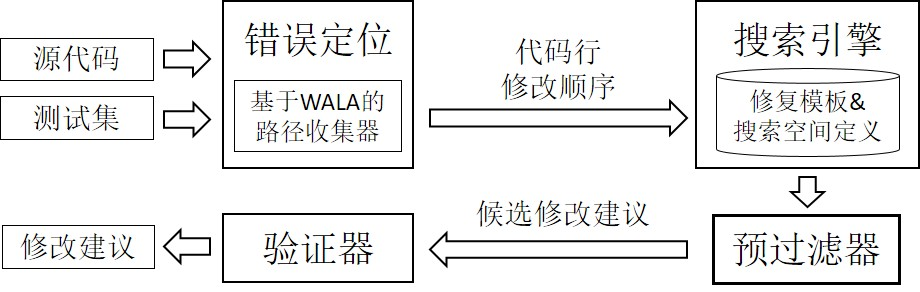
\includegraphics[width=0.6\paperwidth]{chap03/pfstructure}
	\caption{PfDebug的系统结构}
	\label{fig:pfstructure}
\end{figure}

Defects4J是“生成-检验”系统常用的程序测试集,它包含5个实际程序的357个版本,每个版本都包括完整的源代码和测试集,且至少有一个可以被检测到的错误。表\ref{tab:defects4J}展示了测试集的基本信息。Defects4J中的程序版本都是实际开发过程中提交的版本,其中的错误修改方式也比较复杂,现有的“生成-检验”系统能够覆盖的范围非常有限。PFDebug的搜索空间能够覆盖其中31个版本,但在系统实现过程中在Java语言处理上存在一些细节问题,(例如Java内部类的字节码与源代码对应问题,循环太多导致插桩后程序运行速度过慢等),系统最终能够修复的版本数为24个。这是目前为止在此测试集上报告的最高数目。

表\ref{tab:pf effect}展示了成功修复的24个版本程序在修复过程中与预过滤效果相关的运行数据:

\begin{table}[!b]
	\centering
	\caption{Defects4J测试集基本信息}
	\label{tab:defects4J}
	\begin{tabular}{|l|c|c|c|c|c|c|c|}
		\hline
		程序名          &代号            & 版本数 & 成功数 & \begin{tabular}[c]{@{}c@{}}代码行数\\ (千行)\end{tabular} & \begin{tabular}[c]{@{}c@{}}测试代码行数\\ (千行)\end{tabular} & 测试数    & \begin{tabular}[c]{@{}c@{}}开发时长\\ (年)\end{tabular} \\ \hline
		JFreeChart      &FC         & 26  & 4     & 96                                                  & 50                                                    & 2,205  & 7                                                  \\ \hline
		Closure Compiler   &CC      & 133 & 11    & 90                                                  & 83                                                    & 7,927  & 5                                                  \\ \hline
		Commons Math     &MA        & 106 & 6     & 85                                                  & 19                                                    & 3,602  & 11                                                 \\ \hline
		Joda-Time        &JT        & 27  & 0     & 28                                                  & 53                                                    & 4,130  & 11                                                 \\ \hline
		Commons Lang     &LA        & 65  & 3     & 22                                                  & 6                                                     & 2,245  & 12                                                 \\ \hline
		\multicolumn{1}{|c|}{总计} & & 357 & 24    & 321                                                 & 211                                                   & 20,109 & -                                                  \\ \hline
	\end{tabular}
\end{table}

\begin{landscape}
% Please add the following required packages to your document preamble:
% \usepackage{multirow}
\begin{table}[]
	\centering
	\caption{预过滤对搜索空间的压缩效果}
	\label{tab:pf effect}
	\begin{tabular}{|l|l|l|l|l|l|l|l|l|l|l|l|l|l|l|}
		\hline
		\multirow{2}{*}{版本号} & \multirow{2}{*}{代号} & \multicolumn{4}{l|}{过滤前}         & \multicolumn{4}{l|}{过滤后} & \multirow{2}{*}{OL/OR} & \multicolumn{2}{l|}{总计} & \multicolumn{2}{l|}{压缩比率} \\ \cline{3-10} \cline{12-15} 
		&                     & EXPR  & BOOL   & CE     & SUM    & EXPR  & BOOL  & ES  & BS  &                         & TOTAL        & VAL         & FULL            & EXPR           \\ \hline
		CC1          &       IB              & 6362  & 256275 & 107674 & 154963 & 860   & 13999 & 291 & 963 & 624                     & 15483        & 1878        & 0.01207         & 0.00809        \\ \hline
		CC10         &       OR              & 19223 & 385645 & 155174 & 249694 & 1778  & 4937  & 118 & 695 & 2783                    & 9498         & 3596        & 0.01424         & 0.00326        \\ \hline
		CC118        &       IB              & 6229  & 468011 & 176216 & 298024 & 491   & 7637  & 76  & 248 & 1311                    & 9439         & 1635        & 0.00546         & 0.00109        \\ \hline
		CC125        &       IC              & 5177  & 347358 & 139623 & 212912 & 141   & 1335  & 5   & 108 & 417                     & 1893         & 530         & 0.00248         & 0.00053        \\ \hline
		CC51         &       IC              & 791   & 4500   & 3479   & 1812   & 0     & 29    & 0   & 4   & 54                      & 83           & 58          & 0.03108         & 0.00221        \\ \hline
		CC62         &       IC              & 4     & 164    & 107    & 61     & 1     & 7     & 1   & 2   & 1                       & 9            & 4           & 0.06452         & 0.04918        \\ \hline
		CC63         &       IC              & 90    & 560    & 323    & 327    & 1     & 7     & 1   & 2   & 77                      & 85           & 80          & 0.19802         & 0.00917        \\ \hline
		CC73         &       IC              & 18    & 4486   & 3452   & 1052   & 0     & 18    & 0   & 4   & 7                       & 25           & 11          & 0.01039         & 0.0038         \\ \hline
		CC86         &       ER              & 556   & 1127   & 814    & 869    & 95    & 166   & 0   & 17  & 160                     & 421          & 177         & 0.17201         & 0.01956        \\ \hline
		CC92         &       OL              & 1479  & 23151  & 7330   & 17300  & 1051  & 2830  & 617 & 654 & 279                     & 4160         & 1550        & 0.08817         & 0.07347        \\ \hline
		CC93         &       OL              & 1479  & 23194  & 7198   & 17475  & 1051  & 2767  & 617 & 642 & 279                     & 4097         & 1538        & 0.08663         & 0.07205        \\ \hline
		LA24            &       ER              & 161   & 1253   & 464    & 950    & 30    & 261   & 7   & 111 & 6                       & 297          & 124         & 0.12971         & 0.12421        \\ \hline
		LA26            &       OL              & 16    & 410    & 113    & 313    & 8     & 89    & 8   & 7   & 43                      & 140          & 58          & 0.16292         & 0.04792        \\ \hline
		LA6             &       ER              & 240   & 385    & 250    & 375    & 68    & 51    & 44  & 21  & 57                      & 176          & 122         & 0.28241         & 0.17333        \\ \hline
		MA75             &       OR              & 3     & 3      & 5      & 1      & 1     & 0     & 1   & 0   & 35                      & 36           & 36          & 1               & 1              \\ \hline
		MA80             &       ER              & 752   & 522    & 241    & 1033   & 519   & 48    & 283 & 8   & 100                     & 667          & 391         & 0.3451          & 0.2817         \\ \hline
		MA82             &       IC              & 295   & 1215   & 806    & 704    & 5     & 42    & 3   & 12  & 80                      & 127          & 95          & 0.12117         & 0.02131        \\ \hline
		MA85             &       IC              & 157   & 238    & 165    & 230    & 0     & 10    & 0   & 3   & 39                      & 49           & 42          & 0.15613         & 0.01304        \\ \hline
		MA33            &       ER              & 790   & 1707   & 970    & 1527   & 3     & 25    & 3   & 10  & 56                      & 84           & 69          & 0.04359         & 0.00851        \\ \hline
		MA5             &       ER              & 12    & 68     & 22     & 58     & 4     & 24    & 4   & 4   & 0                       & 28           & 8           & 0.13793         & 0.13793        \\ \hline
		FC1                &       IC              & 1222  & 7898   & 1488   & 7632   & 873   & 2526  & 816 & 125 & 193                     & 3592         & 1134        & 0.14492         & 0.1233         \\ \hline
		FC11               &       ER              & 56    & 465    & 265    & 256    & 0     & 2     & 0   & 1   & 8                       & 10           & 9           & 0.03409         & 0.00391        \\ \hline
		FC24               &       ER              & 56    & 9      & 11     & 54     & 34    & 0     & 14  & 0   & 26                      & 60           & 40          & 0.5             & 0.25926        \\ \hline
		FC9                &       IC              & 25    & 107    & 71     & 61     & 0     & 1     & 0   & 1   & 3                       & 4            & 4           & 0.0625          & 0.01639        \\ \hline
	\end{tabular}
\end{table}
\end{landscape}


表格第一列是所有成功修复的程序版本编号,对每一个程序版本,我们统计了成功修复改程序所使用的的修复模板(“代号”),在预过滤前系统产生的修复方案数(“过滤前”四列),在过滤后仍被保留的修复方案数(“过滤后”四列),与方法修改相关不参与过滤处理的修复方案数(“OL/OR”),最终需要被检验器检验的修复方案总数(“总计”两列)和搜索空间被压缩的压缩比率(“压缩比率”)。其中,“过滤前”的数据包括四组,分别是:与一般表达式替换相关,即使用模板ER生成的修复方案数(EXPR);与布尔表达式相关,即使用IB,IC,AB,CB,NP,TC模板生成的修复方案数;编译不通过被首先剔除的修复方案数(CE\footnote{由于系统实现时精确的控制表达式的生成过程使得仅生成编译通过的表达式比较困难,因此我们把一部分工作交给了编译器完成,因此会导致CE这一列的出现});与一般表达式和布尔表达式相关的合法修复方案总数(SUM)。“过滤后”也包括四组,分别是:ER产生的修复方案过滤后的剩余数量(EXPR);布尔表达式相关的修复方案过滤后剩余数量(BOOL);ER产生的修复方案划分的等价类数量(ES);布尔表达式相关的修复方案等价类划分数量(BS)。在“总计”这两列中,TOTAL表示过滤后的修复方案总数(EXPR+BOOL),VAL表示需验证的等价类数量(ES+BS)。最后“压缩比率”这两列中,FULL表示把方法相关的修复方案考虑在内,修复方案数在过滤后与过滤前的比值,EXPR表示仅考虑一般表达式和布尔表达式相关的修复方案在过滤后与过滤前的比值。

从最终的压缩比率看,由于每个程序版本修复过程中生成的方法修复数都比较少,因此无论是否将其考虑进来(FULL/EXPR),过滤后需要被检验器验证的修复方案数远小于过滤前。在比较复杂的Closure Compiler程序上,搜索空间巨大,此时预过滤的效果体现的尤其明显,过滤后检验器的工作负担通常仅有过滤前的不超过5\%,在版本号1,10,118,125,51上,这一比率甚至低于1\%。对于较简单的程序,过滤效果虽然没有在Closure Compiler上明显,但这一比率也在10\%-20\%左右。值得一提的是,布尔表达式相关的修复方案数确实占了修复方案总数的绝大部分,这是由于生成一个布尔表达式比较容易,但生成一个同类型的一般表达式则相对困难。在压缩效果上,布尔表达式的压缩比率更小一些,这可能也是SPR专注于If条件搜索优化的一个原因。但是,一般表达式的修复方案也占了一定的比例,而且其数目远远超过最终过滤后的修复方案总数。例如Closure Compiler 10对应的一般表达式修复方案有19223个,如果不对这部分修复方案压缩,那么检验器的工作负担最少是19223,远超过过滤后的3596个。这也说明,在研究搜索优化技术时将一般表达式替换考虑进来是很有必要的。


表格\ref{tab:pf_vs_others}  汇总了在Defects4J测试集上的其他工作的实验结果实验结果。参与比较的系统包括本文实现的PFDebug(PF),Nopol、针对Java版本重新实现的GenProg(jGP)和Kali(jKali)(实验结果来自\cite{Nopol_and_others})。另外我们从搜索空间是否覆盖正确修复建议的角度比较了若实现一个java版本的SPR其可能的实验结果。

表格以\textbullet 表示某系统能够正确修复某版本的程序。defects4J中共有357个版本,PFDebug总共可以修复24个版本。在\cite{Nopol_and_others}的实验中作者只测试了不包括Closure Compiler的其他4个程序共227个版本,因此Nopol,jGenProg和jKali在Closure Compiler上没有实验结果。PF在所有Closure Compiler程序上可以修复11个程序版本。在其余的程序版本上,PFDebug可以成功修复共13个程序版本,而Nopol、jGenProg和jKali最多只能修复5个程序。一个可能的解释是这三个系统没有使用有效的搜索空间压缩手段,所以无法覆盖较大的搜索空间,修复正确率也比较低。

此外,我们分析SPR的搜索空间,预测它在其余几个系统能够成功修复的程序上的修复效果。不考虑具体实现,SPR可以修复其中的11个程序,主要原因是SPR的搜索空间只包含了简单语句的一般表达式替换,没有包含方法替换。Java语言中简单表达式较少,方法的重写和重载也比较常见,因此直接将SPR的搜索空间平移到Java语言程序中会有一定的问题。但SPR的搜索空间覆盖范围内能够产生的正确程序修复方案也超过了其他三个系统,这也是SPR优化搜索算法优化效果体现。

\begin{table}
	\centering
	\caption{修复成功率对比}
	\label{tab:pf_vs_others}
	\begin{tabular}{|l|l|l|l|l|l|l|l|l|l|l|l|}
		\hline
		版本    & PF          & Nopol       & jGP & jKali & SPR         & 版本   & PF          & Nopol       & jGP         & jKali       & SPR         \\ \hline
		CC1   & \textbullet &             &     &       & \textbullet & LA58 &             & \textbullet &             &             &             \\ \hline
		CC10  & \textbullet &             &     &       &             & MA5  & \textbullet &             & \textbullet &             &             \\ \hline
		CC51  & \textbullet &             &     &       & \textbullet & MA33 & \textbullet &             &             &             &             \\ \hline
		CC62  & \textbullet &             &     &       &             & MA50 &             & \textbullet & \textbullet & \textbullet &             \\ \hline
		CC63  & \textbullet &             &     &       &             & MA53 &             &             & \textbullet &             & \textbullet \\ \hline
		CC73  & \textbullet &             &     &       &             & MA70 &             &             & \textbullet &             &             \\ \hline
		CC86  & \textbullet &             &     &       &             & MA73 &             &             & \textbullet &             &             \\ \hline
		CC92  & \textbullet &             &     &       &             & MA75 & \textbullet &             &             &             &             \\ \hline
		CC93  & \textbullet &             &     &       &             & MA80 & \textbullet &             &             &             &             \\ \hline
		CC118 & \textbullet &             &     &       & \textbullet & MA82 & \textbullet &             &             &             & \textbullet \\ \hline
		CC125 & \textbullet &             &     &       & \textbullet & MA85 & \textbullet &             &             &             & \textbullet \\ \hline
		LA6   & \textbullet &             &     &       & \textbullet & FC1  & \textbullet &             &             &             & \textbullet \\ \hline
		LA24  & \textbullet &             &     &       &             & FC5  &             & \textbullet &             &             &             \\ \hline
		LA26  & \textbullet &             &     &       &             & FC9  & \textbullet &             &             &             & \textbullet \\ \hline
		LA44  &             & \textbullet &     &       &             & FC11 & \textbullet &             &             &             &             \\ \hline
		LA55  &             & \textbullet &     &       & \textbullet & FC24 & \textbullet &             &             &             &             \\ \hline
	\end{tabular}
\end{table}


\section{预过滤算法的局限性}

实验结果显示,预过滤算法对搜索空间的压缩效果非常显著,但是在算法实现中我们用到了大量基于经验假设的设计,而非严格的理论推导。例如,在已通过的测试用例执行过程中,替换表达式的值与目标表达式不同不一定会导致已通过的测试用例运行失败。此外,两个表达式取值等价性的判断标准对类对象实例也是比较粗糙的。这两点导致算法有时会将合理的替换表达式滤除掉,系统最终错过了正确的修复建议。

\begin{lstlisting}[caption=错误示例 commons-lang59/StrBuffer.java,frame=single,language=Java,numbers=left,basicstyle=\ttfamily\footnotesize,label={code:lang59}]
//------ source code--------------------------------------------
public StrBuilder appendFixedWidthPadRight(Object obj, int width,
    char padChar) {
  if (width > 0) {
    ensureCapacity(size + width);
    String str = (obj == null ? getNullText() : obj.toString());
    int strLen = str.length();
    if (strLen >= width) {
      //此处strLen -> width
      str.getChars(0, strLen, buffer, size);
    } else {
      int padLen = width - strLen;
      str.getChars(0, strLen, buffer, size);
      for (int i = 0; i < padLen; i++) {
        buffer[size + strLen + i] = padChar;
      }
    }
    size += width;
  }
  return this;
}

//------ test code--------------------------------------------
public void testAppendFixedWidthPadRight_int() {
  StrBuilder sb = new StrBuilder();
  sb.appendFixedWidthPadRight(123, -1, '-');
  assertEquals("", sb.toString());  
  ...
}

// See: http://issues.apache.org/jira/browse/LANG-299
public void testLang299() {
  StrBuilder sb = new StrBuilder(1);
  sb.appendFixedWidthPadRight("foo", 1, '-');
  assertEquals("f", sb.toString());
}
  
\end{lstlisting}

例如,在代码\ref{code:lang59}中,被测对象是\texttt{StrBuffer}类中的方法\texttt{appendFixedWidthPadRight},方法的功能是在当前\texttt{StrBuffer}对象的字符缓冲区右端附加对象obj转换的字符串,要求附加的长度为width,不足的部分用\texttt{padChar}补齐。在代码第9行,调用方法\texttt{getChars}时第二个参数应当是\texttt{width},表示截取的是前面\texttt{width}个字符,但误写成了\texttt{strLen},这导致虽然\texttt{StrBuffer}对象表示\texttt{buffer}长度的\texttt{size}属性是正确的,但是\texttt{buffer}数组在超过\texttt{size}的位置上仍有字符。这个错误在上一版本程序中并没有暴露出来,原因是测试代码只包含了类似\texttt{testAppendFixedWidthPadRight\_int()}的测试,由于\texttt{StrBuffer}类重写了\texttt{toString()}方法,虽然\texttt{buffer}数组在超过\texttt{buffer}长度的位置仍有字符,但\texttt{assertEquals}只会对
\texttt{StrBuffer}中不超过buffer长度的字符做判断,于是测试会通过。在下一个版本中,一个专门的测试用例\texttt{testLang299}被加入了测试集,这一问题才被暴露。

当“生成-检验”系统使用预过滤策略时,搜索空间中存在将\texttt{strLen}替换为\texttt{width}的修改方案,然而显然很多情况下\texttt{strLen}和\texttt{width}的值并不相等,于是这一方案被过滤掉了。在这一版本程序中我们没有发现更好的等价修复方案,因此最终PFDebug无法成功的修复该版本程序。

在现有预过滤算法的框架下,这一问题可能比较难解决。一种可能的解决思路是引入静态分析技术(如符号执行等),分析将\texttt{strLen}替换成\texttt{width}之后对测试用例结果的影响。事实上SemFix等算法的思路也是如此。但是按照现在的技术发展情况,按这一思路实现的系统计算量较大,速度较慢,可能无法处理Closure Compiler类似规模的程序。



\section{本章小结}%1
“生成-检验”系统的核心模块是搜索引擎。如何定义搜索空间的范围、设计搜索算法,平衡搜索速度与范围之间的关系是搜索引擎设计的关键问题。在本章中,我们分析了现有工作的搜索空间和搜索算法设计方案,借鉴了SPR等工具将搜索模板系统与搜索空间压缩技术相结合的设计思路,提出了“预过滤”搜索算法。算法利用“已通过的测试用例仍应通过,未通过的测试用例执行过程应有变化”这一观察,对搜索模板系统中与表达式修改相关的搜索模板所生成的修复方案进行过滤处理。此外,算法的具体实现利用表达式值的等价关系将搜索空间以等价类结构组织起来,进一步缩减检验模块的工作量。

基于预过滤算法,我们实现了“生成-检验系统”PFDebug。在Defects4J上的测试结果表明,检验模块的工作量减少到了过滤前的10\%-20\%左右,对于规模较大搜索空间复杂的程序(如Closure Compiler)等,搜索空间被压缩到了原来的1\%以下。与现有的其他工作相比,PFDebug能够成功修复其中24个程序,修复正确率超过Nopol,jGenProg,jKali等现有系统。